\setcounter{chapter}{3}
\setcounter{section}{0}

\chapter{Mansioni}
        \par
            La seguente sezione illustra la suddivisione delle mansioni svolte durante il periodo del tirocinio curricolare. Generalmente si possono distinguere gli interventi di \textit{Collaborazione alla gestione Informatica e Multimediale}, gli interventi di \textit{Manutenzione degli Impianti Informatici e Audiovisivi di un Polo Universitario} e infine alcuni interventi di natura generale, non riconducibili alle due categorie sopra elencate. 
% ---------------------------------------------------------------------------------------
        \section{Collaborazione alla gestione Informatica e Multimediale}
            \par
                Gli interventi principali di Collaborazione alla Gestione Informatica riguardano gli aggiornamenti software dei vari computer comprendendo quelli in uso all'Amministrazione, quelli in uso alla Biblioteca, quelli presenti nei Laboratori di Informatica 1 e 2 e quelli in uso ai Docenti. Tutti questi computer operano sulla versione 25H2 di Windows Enterprise, permettendo una copertura da patch della sicurezza future. I due Laboratori di Informatica hanno una trentina di computer ciascuno e ognuno di questi è configurato per poter permettere l'accesso al proprio account tramite Server di Autenticazione RADIUS gestito dall'Università degli Studi di Udine. L'account di accesso ha le stesse credenziali del proprio account istituzionale (\emph{spes.uniud.it}). Una nota di apprezzamento va espressa nei confronti degli impianti di entrambi i laboratori: questi due operano sulla stessa VLAN in modo da poter permettere una comunicazione tra tutti i computer; i Laboratori inoltre presentano una telecamera che inquadra la postazione docente offrendo la possibilità di trasmettere il flusso video nell'altro laboratorio, tramite uno schermo dedicato.  \newline
                Ogni computer ha la possibilità di accedere con un account locale con privilegi di amministratore, ma questo viene utilizzato esclusivamente per l'installazione e la configurazione di software richiesto dal Corpo Docenti o per poter eseguire interventi di manutenzione straordinaria. 
            \par
                La collaborazione alla gestione informatica comprende anche il supporto informatico e multimediale per tutta la durata di eventi, di convegni e di symposium. Prima del loro inizio si verifica la stabilità dell'impianto e il corretto funzionamento dei microfoni e delle casse stereo, predisponendo poi due computer in modo da registrare audio e video dell'evento intero per fornirlo quindi agli studenti che ne richiedono l'accesso durante l'evento stesso in modo da fornire supporto immediato. Ad evento terminato si spegne l'impianto e si verifica lo stato della registrazione completa; non appena questa viene elaborata dai server di Teams, si prevede il caricamento sui canali ufficiali. \newline
                Nel caso i Relatori di un evento abbiano anticipato alla Direzione della necessità di un collegamento su Teams, si predispone la chiamata tra il Relatore o Relatrice connessi e i restanti presenti nell'aula, in modo che chi sia connesso possa seguire la durata dell'intero evento e intervenire al momento ritenuto opportuno. 
            \par
                Durante il primo semestre si sono svolti i Test d'Ingresso per il Corso di Laurea in Relazioni Pubbliche. Il compito svolto riguardava la predisposizione dei computer presenti nei due Laboratori di Informatica, avviandoli, accedendo ad un account dedicato e lanciando il software Safe Exam Browser (SEB) dato che i Test offrono una correzione automatica al loro termine. Mentre gli studenti eseguivano i test, la presenza del sottoscritto è stata fondamentale in quanto ne fornisce supporto immediato ai problemi che si sono verificati. \newline
                Durante una sessione dei Test d'Ingresso, ho segnalato a chi di competenza due computer desktop che hanno avuto problemi. Rispettivamente un computer aveva problemi di natura hardware in quanto non riscontrava alcun segnale video nonostante il monitor fosse collegato al computer, mentre l'altro dispositivo aveva problemi di natura software, in quanto SEB mostrava una finestra di dialogo con un errore riferito alla mancata presenza del file di configurazione.
% --------------------------------------------------------------------------------------       
            \subsection{Configurazione Tablet}
                La Prof.ssa Pocecco, referente del Dipartimento di Lingue e Letterature, Comunicazione, Formazione e Società (DILL), ha acquistato una decina di tablet Samsung Galaxy Tab A7 destinati a progetti proposti a studenti. Questi tablet, acquistabili solo da aziende ed enti certificati, sono ottimi per una connessione On-The-Go (OTG) a riunioni online, fornendo un ottimo e accessibile supporto informatico e digitale. \newline
                Solamente alcuni dispositivi erano stati configurati in precedenza all'avvio del Tirocinio e mi sono occupato quindi di inizializzarli tramite il processo di setup iniziale di Android e, una volta terminato, di predisporli completamente all'uso. \newline
                Per poterli configurare in maniera il più possibile simile al login dei computer dei Laboratori di Informatica 1 e 2 ho dapprima disinstallato tutte le app di servizi terzi non utili ai fini dei vari tablet, del tipo Netflix, Amazon e altre applicazioni simili; successivamente ho limitato l'uso di altre applicazioni disabilitandone il servizio, quale per esempio l'accesso a Gmail. Infine ho suggerito alla Direzione di creare un account Google necessario per poter  installare l'applicazione \textsl{Boot Apps}, la quale permette l'avvio automatico di qualsiasi applicazione e servizio, installando e optando per l'avvio automatico della sola app \textsl{Geteduroam}. Ho deciso di seguire questa configurazione dato che il sistema operativo Android 10 OneUI 2.5 non permette l'avvio automatico di app a meno che non siano di sistema. \textsl{Geteduroam} così facendo, si trasforma in una sorta di setup guidato che permette la configurazione e successiva connessione alla rete \textsl{Eduroam}; l'app necessita di una prima connessione ad Internet per potersi connettere al server RADIUS disponibile all'interno dell'Università. Una volta che ci si è accreditati tramite il proprio utente istituzionale, la connessione Internet precedente non è più essenziale. \newline
                Un'ulteriore serie di applicazioni installate sono legate alla suite di Microsoft, comprendendo Word, Excel e Teams. \newline
                Data l'amplia base di utenti a cui saranno destinati i tablet e la distribuzione che deve essere prima concessa dalla Prof.ssa Pocecco, si è deciso di non inserire alcuna password d'accesso in modo da poterli utilizzare con facilità. Tutt'ora questi dispositivi sono utilizzati durante le riunioni della Direzione per prendere appunti e per seguire collegamenti su Teams. 
% -------------------------------------------------------------------------------------- 
            \subsection{Gestione degli eventi}
                \par
                    Come descritto in precedenza, il supporto informatico e multimediale è esteso anche alla gestione degli eventi. Questo supporto, oltre a coprire la durata degli eventi stessi, si traduce nel tenere aggiornato il calendario degli eventi stessi, per poi comunicarlo a chi di competenza. Questa scaletta era prima mantenuta in un foglio di calcolo Excel condiviso contenete una tabella con i campi più importanti quali titolo, data, ora, descrizione; per poter aggiornare il file, bisognava modificare i permessi di condivisione; dato che esso era di proprietà di un ex collega, si è optato per la creazione di un altro file, basato sul foglio di calcolo condiviso, in modo da poter archiviare il precedente, ormai obsoleto. \newline
                    Dopo una riunione con alcuni rappresentati della Direzione del CEGO, si è deciso di migrare questo file alla piattaforma online Microsoft Planner, creando diversi contenitori dove si inserivano le varie attività e gli eventi da poter poi aggiornare "in corso d'opera".
                \par 
                    Microsoft Planner ha permesso alla Direzione di avere una maggiore visione d'insieme per quanto riguarda tutte quelle tipologie di eventi e di compiti assegnati ai vari membri del personale. Nello specifico uno di questi contenitori riguardava gli interventi programmati di manutenzione informatica e una parte di formazione del personale, approfondita in seguito. 
                    L'intervento programmato più pressante riguardava l'aggiornamento e la riconfigurazione di rete dei vari dispositivi mobili, quali i portatili per i Docenti, i tablet e i portatili della Direzione, con le nuove impostazioni di sicurezza della rete \textsl{Eduroam}. \newline
                    L'aggiornamento è avvenuto senza problemi per i tablet, in quanto non richiedevano alcuna credenziale di amministratore; per i portatili della Direzione invece è stato richiesto l'intervento del Dott. Castelli per poter lanciare l'eseguibile di configurazione con permessi superiori. Infine, per quanto riguarda i portatili in dotazione ai Docenti, si è deciso di non aggiornare alle nuove impostazioni di sicurezza in quanto essi sono principalmente collegati ad Internet tramite connessione cablata, garantita dall'Università e presente in ogni aula e Studio Docenti. 
% --------------------------------------------------------------------------------------
            \subsection{Gestione dei CFU soprannumerari degli Studenti}
                 \par
                    In relazione alla gestione degli eventi, ognuno di questi rilasciava agli studenti partecipanti un attestato soprannumerario con valenza di 0,25 CFU, 0,50 CFU o più raramente 0,75 CFU. Per tenerne traccia la Segreteria studentesca del CEGO ha utilizzato un foglio di calcolo Excel. Questo file era stato concepito per la semplice catalogazione e l'aggiornamento di ogni singola carriera degli studenti in modo da fornire un calcolo dei CFU soprannumerari a fine carriera. Il compito assegnatomi riguardava la semplificazione del file precedente per renderlo più accessibile, mantenendo i dati già inseriti e prevedendo l'aggiunta dei vari certificati futuri. \newline
                    Il file è una sorta di database delle carriere studentesche composto da quattro tabelle di cui una è pivot: la prima tabella contiene i dati anagrafici degli studenti (matricola, cognome, nome, corso); la seconda tabella contiene nome e data degli eventi, estrapolati dal file di organizzazione precedentemente citato, e il valore del certificato dell'evento; la terza tabella mette in relazione gli studenti con gli eventi cui hanno partecipato con l'inserimento di sola matricola e nome dell'evento seguito; l'ultima tabella è di tipo pivot ed è risultante dalla relazione precedente, fornendo la somma dei CFU ottenuti dai vari corsi associata ai dati dello studente o studentessa. \newline
                    Logicamente, queste tabelle operano come un database la cui relazione tra i dati degli studenti e gli eventi si traduce in una relazione uno a molti\footnote{"Il sottosistema GD", \cite{sciutoIntroduzioneAiSistemi2022}}, ovvero che uno studente, con matricola univoca, può e ha seguito almeno un evento e quindi, nella tabella degli eventi seguiti, la sua matricola comparirà più di una volta. \newline
                    Si è deciso di mantenere l'organizzazione del calcolo dei CFU soprannumerari in un file Excel in quanto offre un'accessibilità maggiore a tutto il personale, senza dover installare e mantenere un server SQL o Access all'interno del server presente nel Centro Stella.
% ---------------------------------------------------------------------------------------
            \subsection{Formazione del personale in merito agli Impianti Informatici e Multimediali}
                    Come citato in precedenza, mi sono occupato anche di formare il personale, distinguendo la formazione in due gruppi differenti, create sulla base dell'obiettivo e il target: la prima categoria comprende i Tutor e i nuovi tirocinanti mentre la seconda comprende il personale esterno della Portineria. 
                \par
                    Per quanto riguarda i Tutor e i nuovi tirocinanti, la formazione ha incluso una parte di illustrazione di collegamento agli impianti e una carrellata di problemi che si possono verificare, come per esempio la mancanza del segnale video sul proiettore. Inoltre ho fornito supporto alla condivisione e alla produzione di grafiche basate anche sulla nuova identità visiva dell'Università, installando il font \textsl{Work Sans} e impostandolo come predefinito per i nuovi modelli dell'identità visiva. \newline
                    L'obiettivo di questa formazione è stato rendere i Tutor più autonomi in caso di assenza del Tecnico durante gli eventi; invece l'obiettivo fissato per i nuovi tirocinanti riguardava più il passaggio di consegne, anche in previsione della fine del mio tirocinio curricolare. 
                \par
                    Per quanto riguarda il personale esterno della Portineria, bisogna sottolineare un primo passaggio di richiesta alla Direzione, la quale ha avuto esito positivo dopo essersi messa in contatto con l'ente esterno Sicuritalia. La formazione, simile a quella per i Tutor e per i nuovi tirocinanti, riguardava per lo più gli impianti: come funzionano sinteticamente e cosa fare in caso di problemi tecnici facilmente risolvibili, soprattutto in relazione al segnale audio e al segnale video. \newline
                    L'obiettivo invece di questa formazione era rendere più efficace l'intervento del Tecnico in caso di problemi gravi agli impianti informatici e multimediali, dato che la maggior parte dei Docenti si interfaccia dapprima con il personale di turno della Portineria che a loro volta contatteranno il Tecnico.
                \par
                    La formazione, indipendentemente dal target e l'obiettivo, è stata basata sul documento "DAGS Formazione Personale 2025" fornitomi dalla Direzione in previsione della fine del mio tirocinio curricolare. 
% ---------------------------------------------------------------------------------------
        \section{Manutenzione degli Impianti Informatici e Audiovisivi di un Polo Universitario}
            \par
                Uno dei compiti assegnatomi è stato quello di mantenere gli impianti informatici e audiovisivi del CEGO in uno stato ad hoc; questo si è tradotto in più interventi mirati alla risoluzione dei problemi tecnici riguardanti tutte quelle problematiche relative al segnale audio e al segnale video, localizzandole alla sola postazione del docente o all'impianto presente nelle aule multimediali. \newline
                La maggior parte di questi interventi si sono svolti durante i primi minuti di ogni blocco ore di lezione, in quanto molto spesso i problemi tecnici si verificavano non appena i Docenti andavano a collegarsi all'impianto audiovisivo con il portatile appositamente a disposizione, oppure il loro computer personale. In questo ultimo caso, tutte le operazioni che sono andato ad eseguire le ho svolte con il Docente a fianco, mostrandogli e illustrandogli apertamente cosa fare, mantenendo il più alto livello di riservatezza e intervenendo solamente se necessario. \newline
                Nel corso del tirocinio, solamente pochi miei interventi hanno richiesto il supporto di un Tecnico Informatico in contratto con l'Ateneo e questi pochi interventi hanno richiesto solamente il reset o la riconfigurazione del controller o del proiettore o, nel peggiore dei casi, la sostituzione del commutatore. 
            \par
                Di seguito vengono elencati quattro interventi ordinati in base alla gravità e durata dell'intervento, oltre all'applicazione della teoria appresa durante il Corso di Studi.
% ---------------------------------------------------------------------------------------
            \subsubsection{Intervento sulla configurazione delle Stampanti}
                    Il primo intervento ha riguardato la configurazione e la predisposizione delle stampanti nuove assegnate ai Laboratori di Informatica 1 e 2. Le stampanti erano precedente installate nei laboratori ma mancavano ancora della configurazione lato software, soprattutto nei vari computer messi a disposizione degli studenti. \newline
                    Queste due stampanti, una per laboratorio, sono usate dagli utenti e quindi devono essere disponibili indipendentemente dalla postazione che decide di usare lo studente. La stampante, inoltre, è stata precedentemente configurata limitando le operazioni eseguibili tramite le impostazioni accessibili dal proprio monitor; questa scelta è stata fatta presumibilmente per questioni di sicurezza e organizzazione dell'impianto. \newline
                    Per poter configurare le stampanti all'interno dei vari computer, ho eseguito l'accesso su ogni computer con l'account utilizzato per i Test d'Ingresso e, su ogni macchina, ho avuto accesso alle impostazioni e ho aggiunto manualmente la stampante del rispettivo Laboratorio. Infine su ogni computer è stata impostata la stampante del proprio laboratorio come predefinita, semplificando ulteriormente il processo di stampa da parte degli studenti.
                \par
                    Le stampanti moderne, come quelle in uso nei Laboratori, offrono la possibilità di creare delle code di stampa virtuali tramite la tecnica dello spooling, tecnica fondamentale nel contesto multi-utente del Laboratorio. Questa tecnica introduce un programma intermediario tra il computer e la stampante, gestendo e organizzando la coda di stampa in modo da poter garantire il servizio ad ogni utente connesso. Onde evitare che ogni utente connesso alla stessa rete dei Laboratori potesse avere accesso alla stampante e quindi intercettasse o alterasse la coda di stampa, si è deciso di gestire gli accessi da una lista (Access Control List) che ne bloccasse l'accesso agli utenti non autorizzati\footnote{"La gestione delle periferiche", \cite{sciutoIntroduzioneAiSistemi2022}}.
% ---------------------------------------------------------------------------------------
    \newpage
            \subsubsection{Intervento sul proiettore in Auditorium Fogar}
                    Il secondo intervento ha riguardato un problema avvenuto al proiettore dell'Auditorium Fogar, presso il Polo di Corso Verdi. Questo proiettore, come ogni altro proiettore presente al CEGO, è collegato ad un controller multimediale presente sulla postazione del docente in aula e si accende comunicando con la tecnica PoE. \newline
                    Il proiettore, connesso sia al ricevitore del controller sia all'alimentazione, non riceveva alcun il segnale video nonostante ricevesse l'impulso di accessione. Dato che in settimana si sarebbe svolto l'evento "Welcome Day" per le matricole iscritte al A.A. 2025/2026 con le autorità del Comune di Gorizia presenti, era essenziale far sì che l'intero impianto multimediale funzionasse correttamente. Dopo un mio primo sopralluogo, in cui ho verificato la connessione di tutti i cavi presenti nella postazione docente, ho verificato poi con un altro dispositivo oltre al computer precedentemente connesso. Dopo più cicli d'avvio, su suggerimento della Direzione, si è deciso di aprire un ticket di assistenza urgente. \newline
                    L'intervento si è svolto nel corso della giornata successiva alla segnalazione del problema al Dott. Barreca con il quale mi sono interfacciato e ho fornito tutti i dettagli necessari affinché si potesse risolvere il problema all'impianto. Per poter meglio isolare l'origine di questo malfunzionamento, io e il Tecnico siamo saliti in regia, dove si trova il ricevitore del controller connesso al proiettore stesso; da qui ci siamo connessi direttamente al proiettore verificando il suo corretto funzionamento, isolando in una prima fase il problema alla comunicazione tra il controller e il suo ricevitore. Successivamente, dopo un ciclo di spegnimento e riaccensione, il proiettore si è "riagganciato" al segnale proveniente dal controller posizionato sulla postazione docente, tornando così alla sua configurazione precedente, risolvendo per tempo il malfunzionamento.
                    %
                \par
                    Per creare il canale di comunicazione tra controller e ricevitore, ma soprattutto per usare la tecnica PoE, è necessario che entrambi questi due dispositivi siano connessi da un cavo di rete Ethernet con rispettiva porta RJ45. Questo cavo è composto da più coppie di cavi, coordinati in base al colore, utilizzati per il collegamento ad Internet; esistono diverse categorie ordinate per velocità e frequenza crescenti, le più comuni sono 5e (Cat. 5 Enchaned), 6 e 7. Tutte queste tre categorie supportano velocità di trasmissione da 1 Gbps fino ai 10 Gbps della Cat. 7 però ne risentono della distanza, soprattutto se questa sfora i 100 metri. La differenza sostanziale tra queste tre categorie è la costruzione fisica del cavo in quanto i cavi di Cat. 5e sono tutti \textsl{Unshielded Twisted Pair} (UTP), i cavi di Cat. 6 sono sia UTP che \textsl{Shielded Twisted Pair} (STP) mentre i cavi di Cat. 7 sono \textsl{Shielded/Foiled Twisted Pair} ovvero che i cavi di Cat. 6 presentano una schermatura solamente attorno alla guaina protettiva più esterna mentre i cavi di Cat. 7 presentano sia una guaina protettiva esterna che una serie di altre guaine protettive intorno ad ogni coppia di doppini\footnote{"Le infrastrutture di rete", \cite{sciutoIntroduzioneAiSistemi2022}}. 
% ---------------------------------------------------------------------------------------
            \subsubsection{Intervento sulla tavoletta grafica in Auditorium Fogar}
                    Anche questo intervento ha riguardato l'Auditorium Fogar e la tavoletta grafica presente su ogni postazione docente del CEGO. La tavoletta è di norma collegata all'impianto tramite cavo HDMI e successivamente collegata al computer tramite cavo USB. Questa doppia connessione permette sia la duplicazione del monitor a cui è collegata sia l'uso dello \textsl{stylus} tramite la connessione USB; come ogni periferica, per poter garantire la più completa compatibilità bisogna installare i driver opportuni, già presenti nei computer dati in dotazione ai Docenti. \newline
                    La tavoletta era già stata precedentemente segnalata tramite il sistema di ticket dell'Università a causa di un apparente guasto al segnale video. Il giorno successivo alla segnalazione, mentre offrivo supporto all'evento "\textsl{Come scrivere una tesi di laurea degna di lode}" tenutosi presso il Polo di Santa Chiara, ho ricevuto una chiamata da parte del Dott. Barreca per poter verificare di persona la veridicità del guasto. \newline
                    Per isolare i vari componenti e quindi meglio identificare il problema che causava la mancanza di segnale video, ho portato un monitor avente anch'esso un'uscita HDMI. L'uso di questo monitor ausiliario ha permesso di circoscrivere il problema allo splitter HDMI (\textit{Figura 4.1}), utile in congiunzione con il controller multimediale, oppure alla tavoletta grafica. Lo splitter HDMI presenta, oltre alla porta di alimentazione, un'entrata HDMI dalla sorgente collegata e due uscite che duplicano tale entrata. \newline
                    Una volta collegato il monitor ausiliario all'alimentazione e all'uscita HDMI presente, ho potuto constatare che il problema poteva riguardare la tavoletta grafica piuttosto che lo splitter stesso; nell'andare a verificare il corretto funzionamento della tavoletta grafica e quindi scollegare il cavo utilizzato al monitor HDMI, ho notato che dallo splitter non vi era alcuna entrata da duplicare sulla tavoletta grafica e che il solo cavo collegato all'impianto del controller era quello presente sulla postazione docente, rendendo lo splitter effettivamente "inutile". \newline
                    Sulla postazione docente dell'Auditorium, il Docente può collegarsi su tre punti diversi, senza andare ad alterare l'impianto stesso: due collegamenti sono sulla postazione mentre l'ultimo è presente sul leggio. Date queste possibilità di collegamento, i cavi di ciascuna sono stati raggruppati in due guaine in maglia espandibile, una per la postazione e una per il leggio, in modo da poter semplificare i collegamenti e facilitare l'eventuale spostamento della postazione docente. Tuttavia ho dovuto ricablare la postazione docente, aggiungendo un cavo HDMI allo splitter, in modo da rendere la tavoletta funzionante, mantenendo intatto il segnale video diretto al proiettore; il cavo HDMI utilizzato era già presente, fissato sotto alla postazione docente con delle fascette adesive, presumibilmente proveniente da una configurazione precedente che contemplava una posizione diversa della tavoletta grafica. \newline
                    Per assicurarmi il funzionamento complessivo dell'impianto, ho eseguito l'intervento con una sorgente video sempre connessa e, ad ogni spostamento di cavo, ricontrollavo la qualità complessiva. Da aggiungere che durante il ricablaggio ho notato una forte interferenza proveniente dall'impianto audio; sono riuscito ad isolare il problema a uno dei microfoni presenti sulla postazione, immaginando un collegamento non corretto ma, una volta acceso singolarmente, l'interferenza persisteva; una volta accertato che il collegamento fosse corretto, ho notato un difetto alla base del microfono stesso che, al minimo movimento, produceva l'interferenza andando a macchiare la qualità audio. \newline
                    L'intervento si è concluso segnalando al Dott. Barreca il corretto funzionamento della tavoletta grafica e dell'impianto intero ma aggiungendo il guasto inatteso del microfono. Su suo suggerimento e grazie alla Direzione, il microfono guasto è stato spedito per posta interna agli uffici del DAGS ai fini di una tempestiva soluzione. 

                    \hfill
                \begin{figure}[htbp]
                    \centering
                    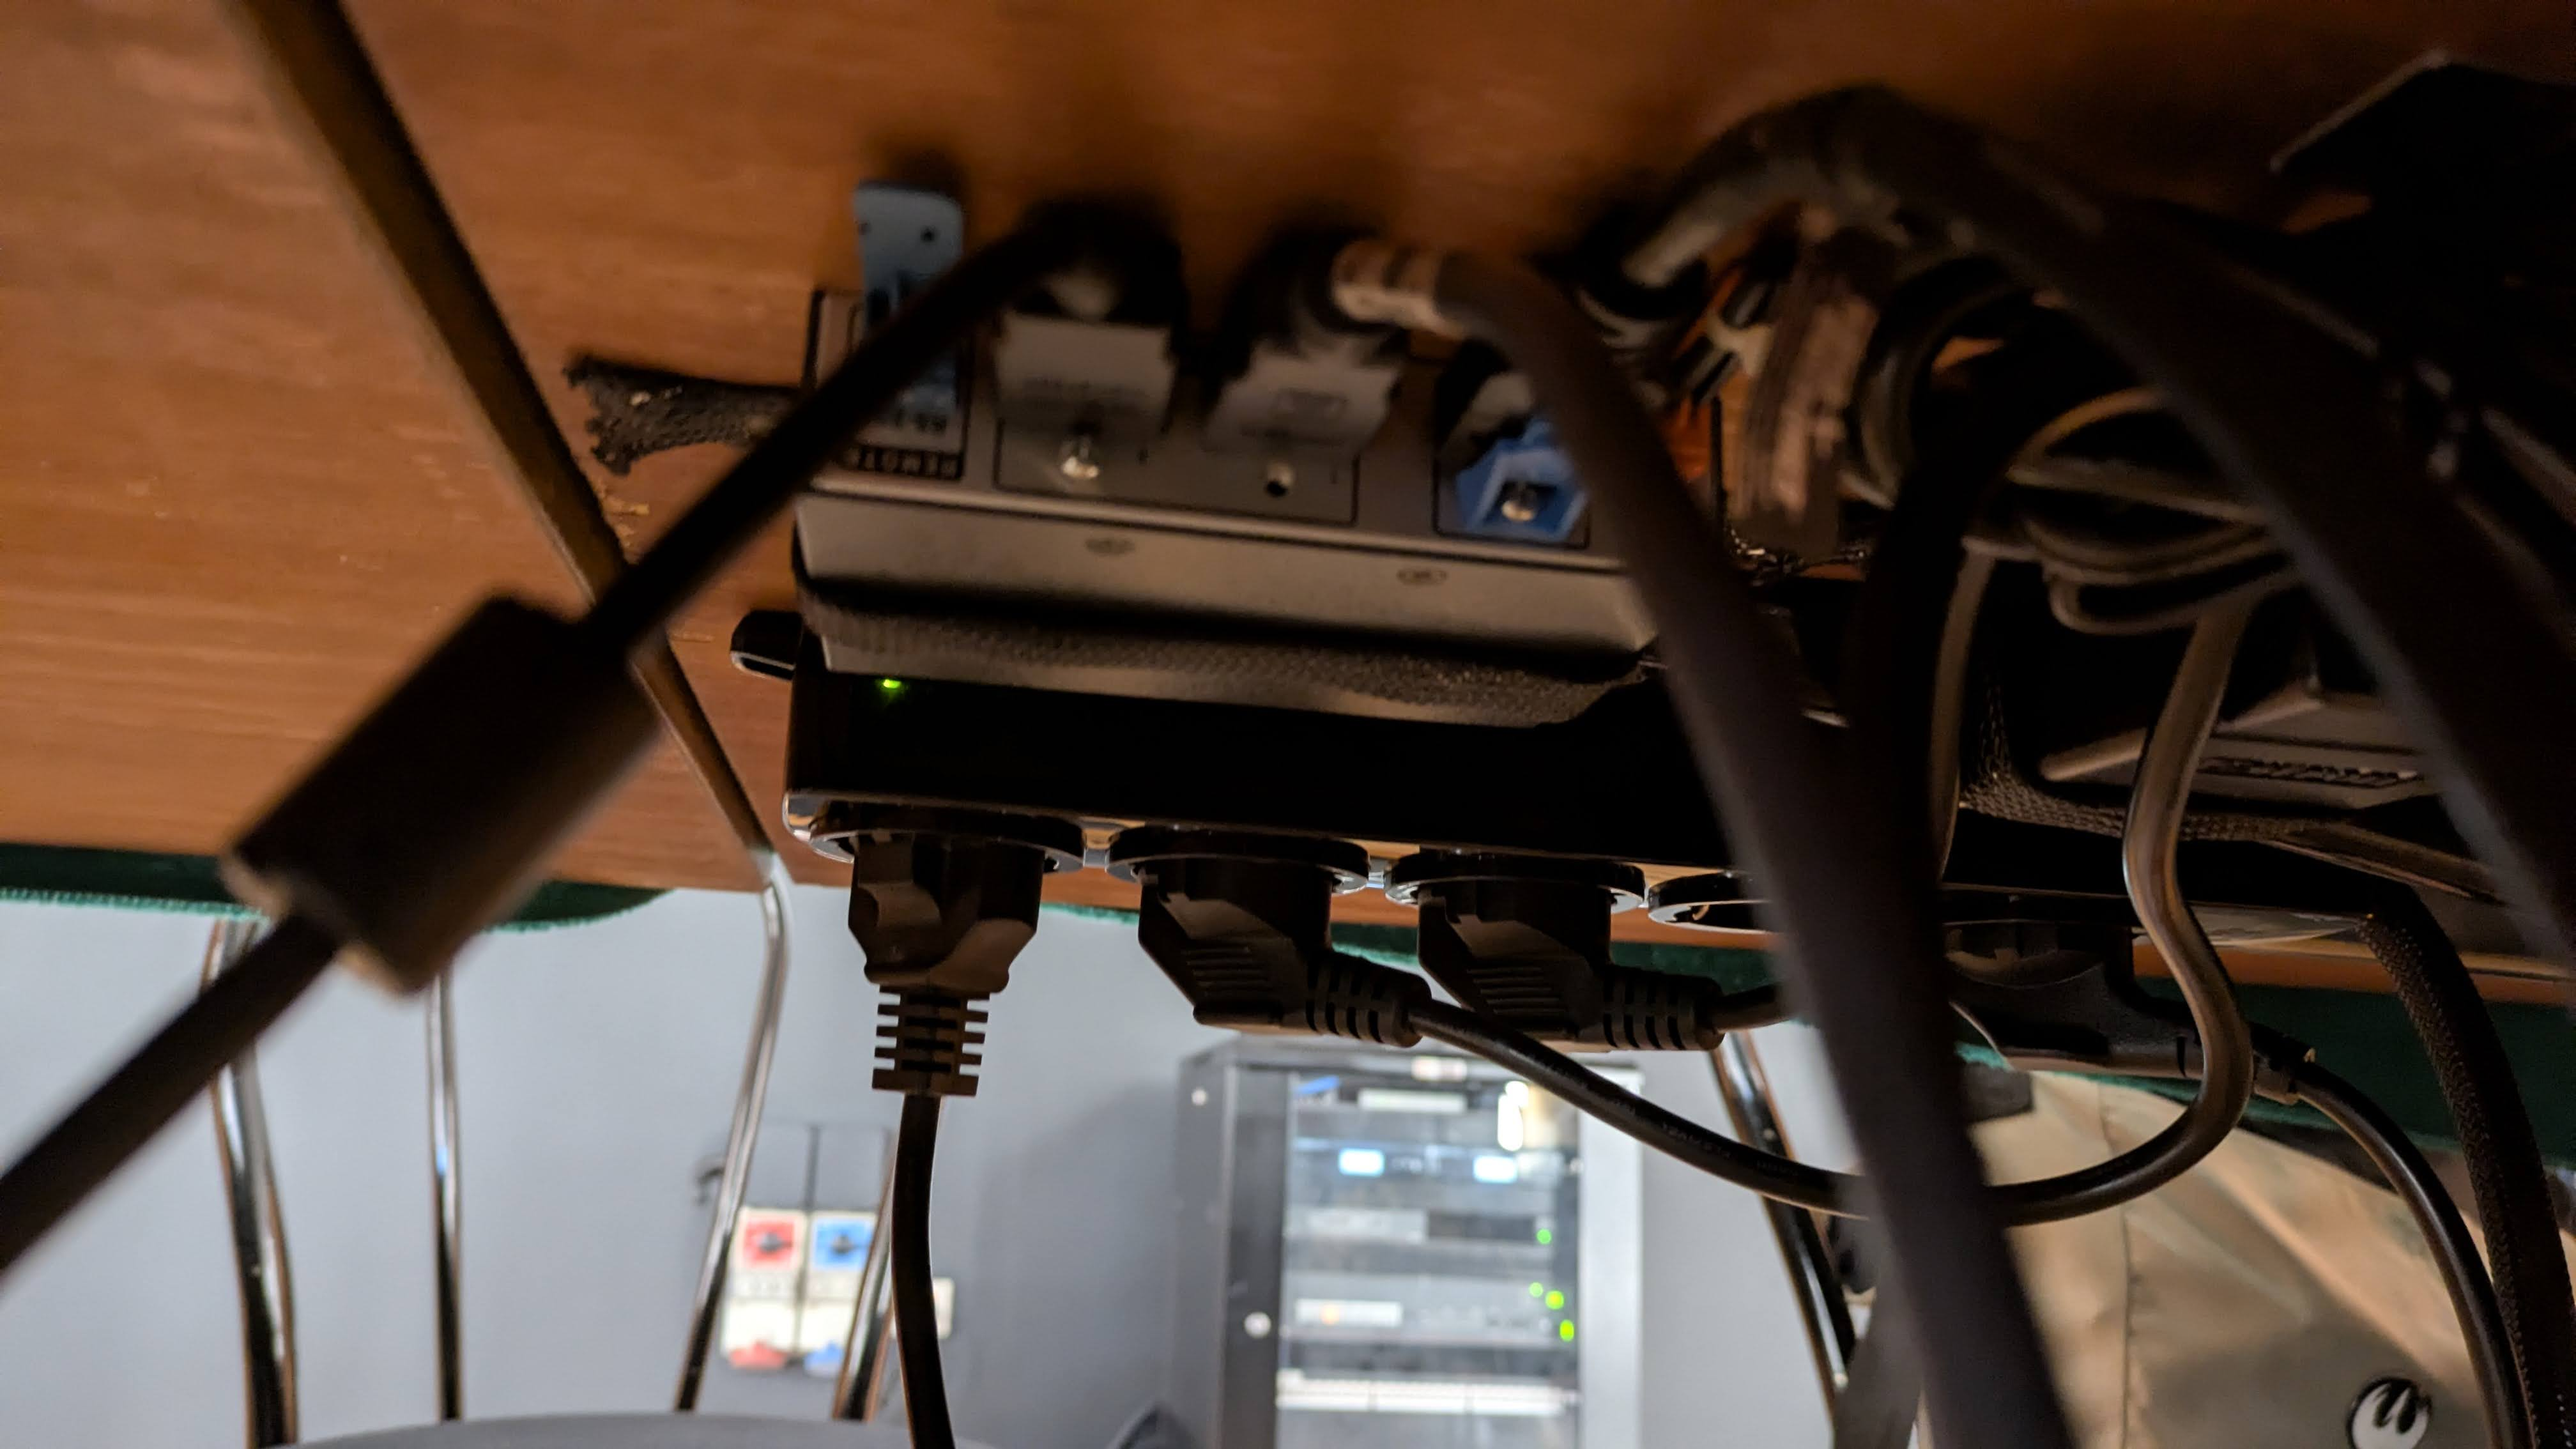
\includegraphics[width=12cm]{imgs/commutatore.jpg}
                    \caption{\textit{Splitter HDMI posto al di sotto della postazione docente}}
                    \label{fig:splitterWacom}
                \end{figure}
        
                \begin{figure}[htbp]
                    \centering
                    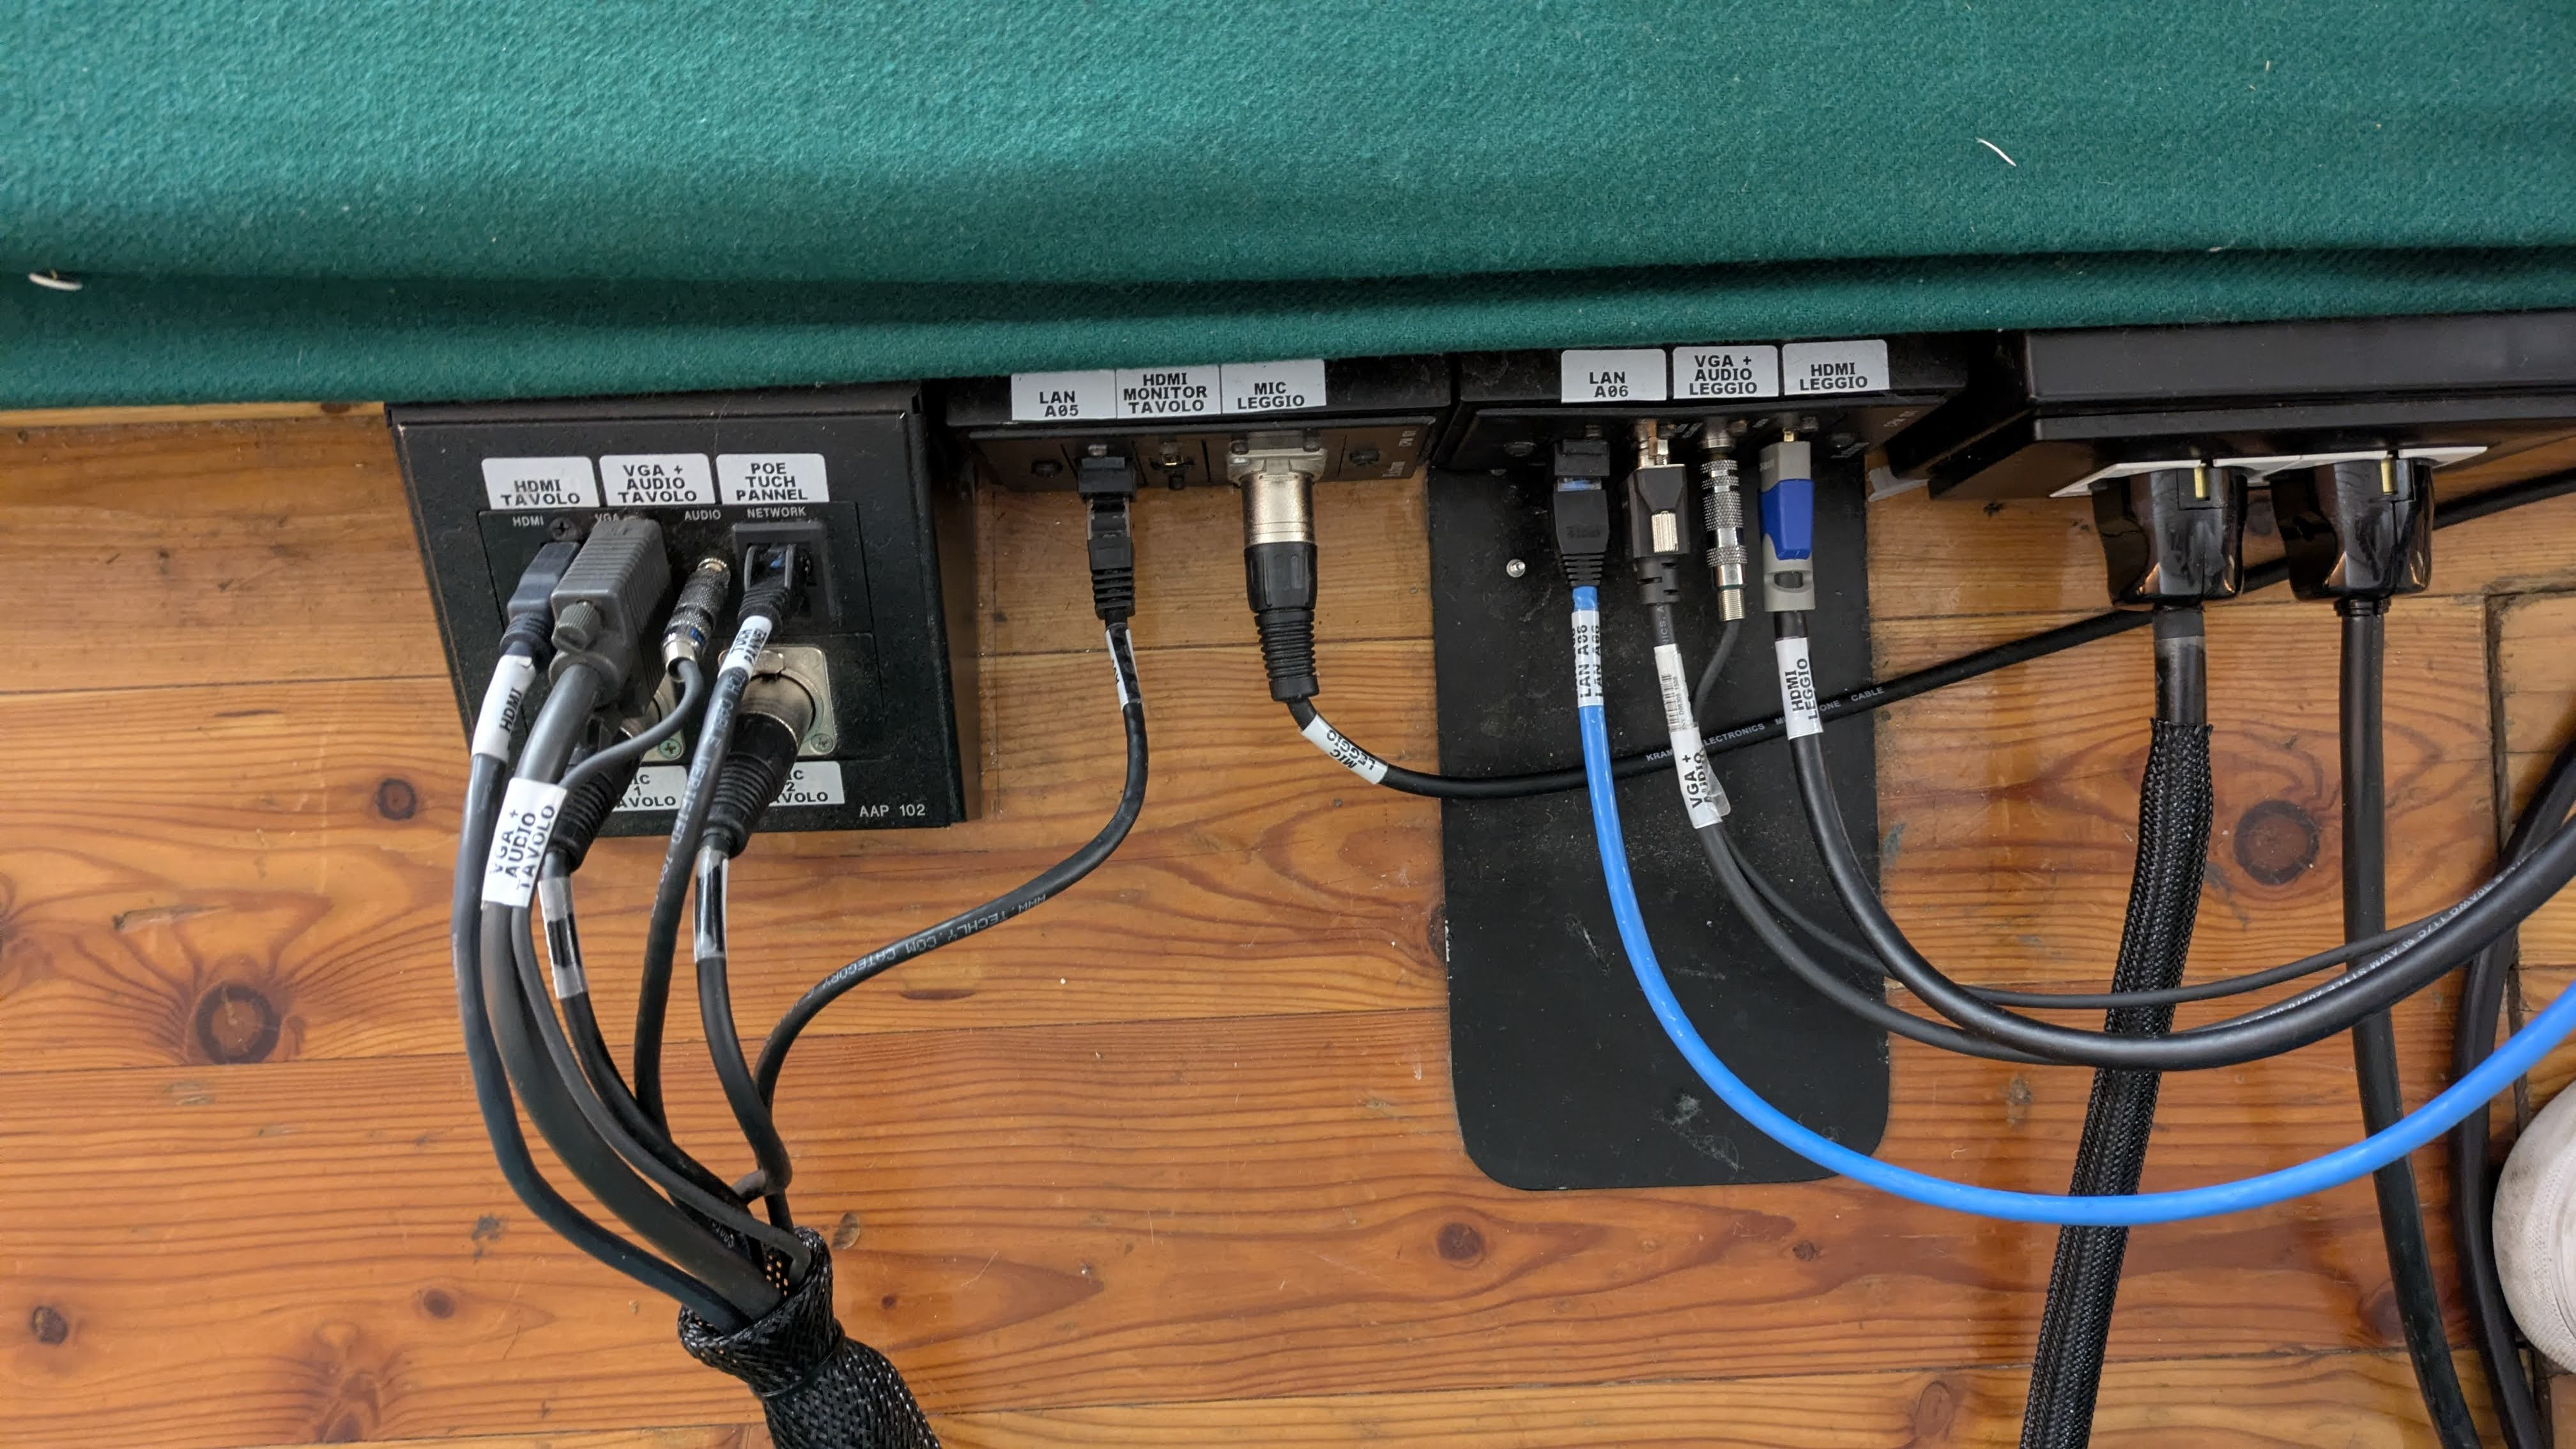
\includegraphics[width=12cm]{imgs/caviPostazione.jpg}
                    \caption{\textit{Cavi della postazione docente all'Auditorium Fogar}}
                    \label{fig:caviFogar}
                \end{figure}
% ---------------------------------------------------------------------------------------
    \newpage
            \subsubsection{Intervento sul proiettore in Aula Magna}
                    Il quarto e ultimo intervento descritto qui riguarda il proiettore presente in Aula Magna, presso il Polo di Santa Chiara. Il proiettore, collegato all'impianto tramite il controller multimediale, è montato a soffitto tramite una struttura apposita e, come ogni altro proiettore presente al CEGO, viene controllato dalla postazione del docente. \newline
                    Durante una lezione pomeridiana, mi è stato segnalato che il proiettore presentava degli artefatti visivi (\textit{Figura 4.3}) quando veniva collegato un portatile in dotazione ai Docenti; data la presunta natura del problema, la soluzione più rapida è stata quella di spostare la lezione in un'altra aula disponibile con impianto funzionante. Dopo numerosi cicli d'avvio e aver verificato se il problema persisteva anche sull'ingresso VGA, ho comunicato alla Direzione la necessità dell'intervento di un altro Tecnico. \newline
                    Questo primo intervento da parte del Tecnico esterno si è tradotto in un reset della configurazione del proiettore tramite il telecomando e, dopo svariati tentativi, gli artefatti visivi si sono risolti; ho chiesto al personale addetto alla Portineria, con cui si è interfacciato il Tecnico per orientarsi all'interno del Polo di Santa Chiara, la conferma della presenza del telecomando del proiettore presente in Aula Magna in caso di problemi futuri. \newline
                    Due giorni dopo l'intervento del Tecnico il problema è riemerso e, dopo un mio primo controllo tramite diversi cicli d'avvio e la verifica di entrambe le sorgenti, ho notato che il problema questa volta compariva anche se ci si collegava tramite l'uscita VGA (\textit{Figura 4.4}); ho contattato la Direzione avvisando del problema riemerso e di come si fosse "espanso" anche all'altro ingresso. Ho suggerito che, nella peggiore delle ipotesi, si dovesse cambiare l'intero proiettore dato che sembrava essere un problema hardware più che software. Il giorno successivo all'apertura del ticket, il Tecnico ha deciso di cambiare il commutatore collegato al controller Extron (\textit{Figura 4.5}) visto il guasto ad entrambe le uscite video; dopo un riavvio dell'impianto e dopo aver verificato il suo funzionamento collegandosi con un computer prima alla sorgente HDMI e successivamente alla sorgente VGA e infine ad entrambe contemporaneamente con due dispositivi diversi, il Tecnico ha rimosso il dispositivo precedente, lasciando il proiettore acceso in modalità stand-by, facendo notare che l'artefatto non comparirà più. 

            \begin{figure}[htbp]
                \centering
                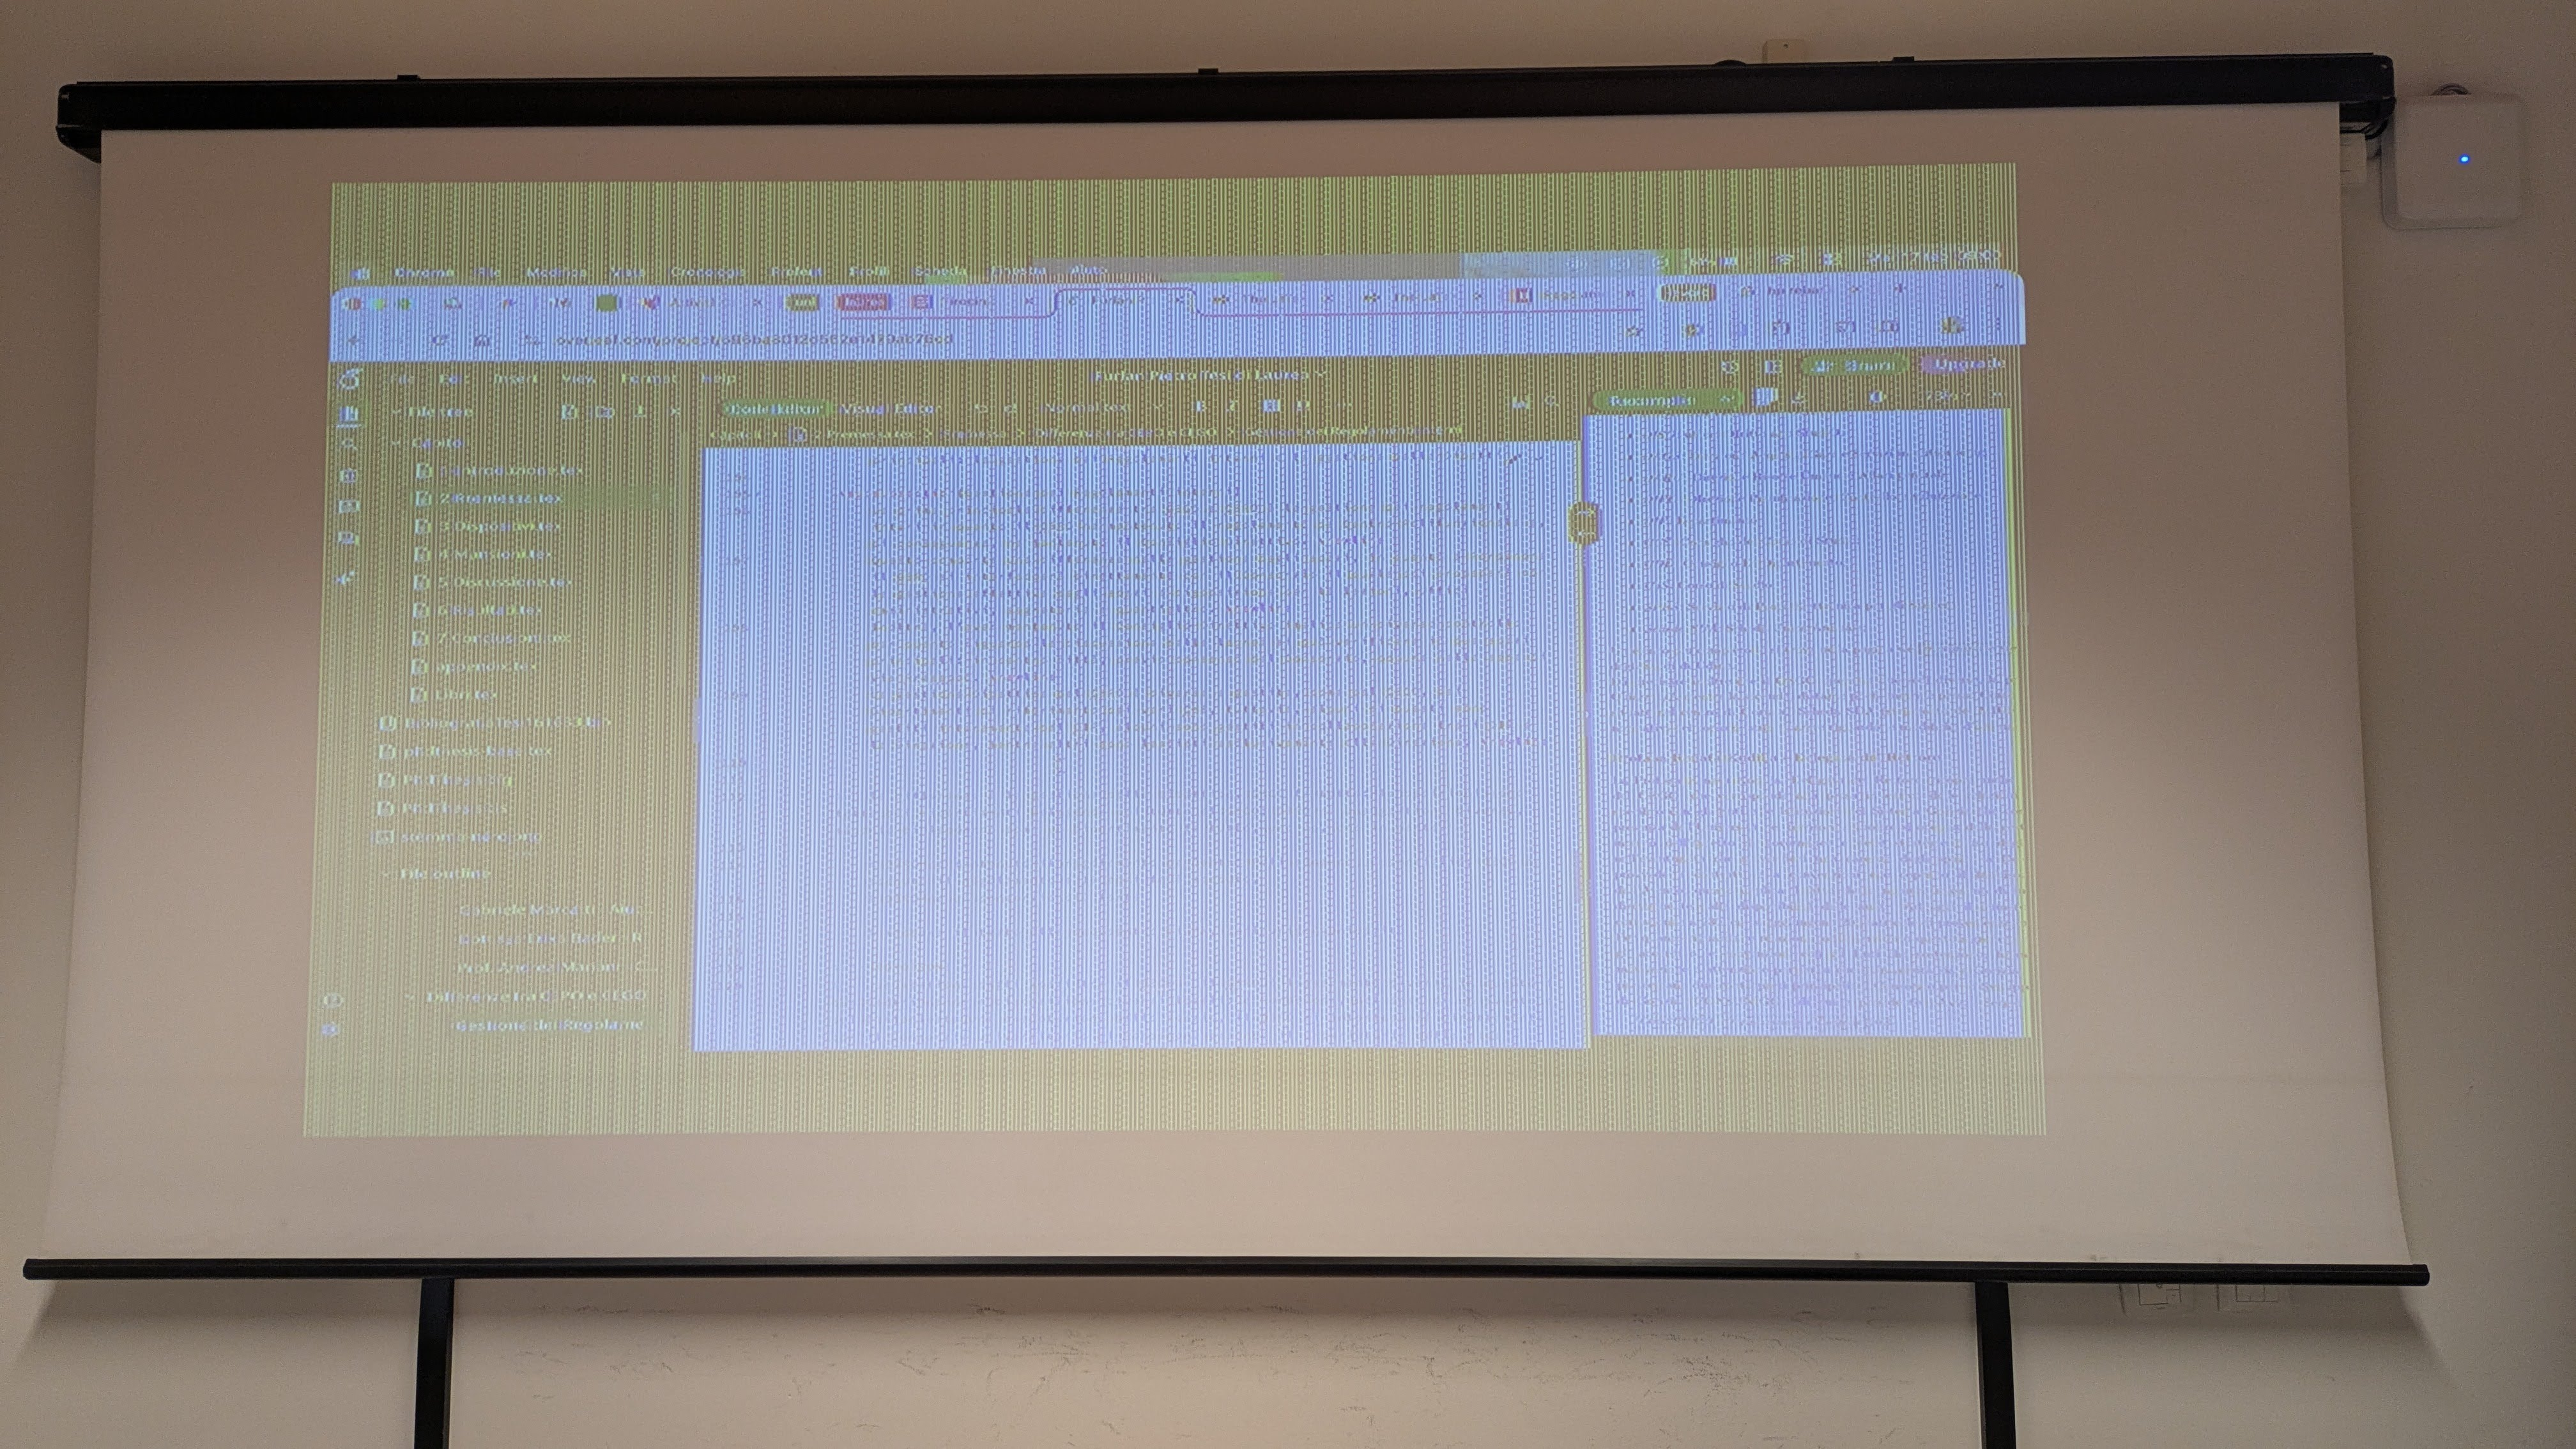
\includegraphics[width=12cm]{imgs/MagnaHDMI.jpg}
                \caption{\textit{Proiettore con collegamento HDMI}}
                \label{fig:HDMIBad}
            \end{figure}
            
            \begin{figure}[htbp]
                \centering
                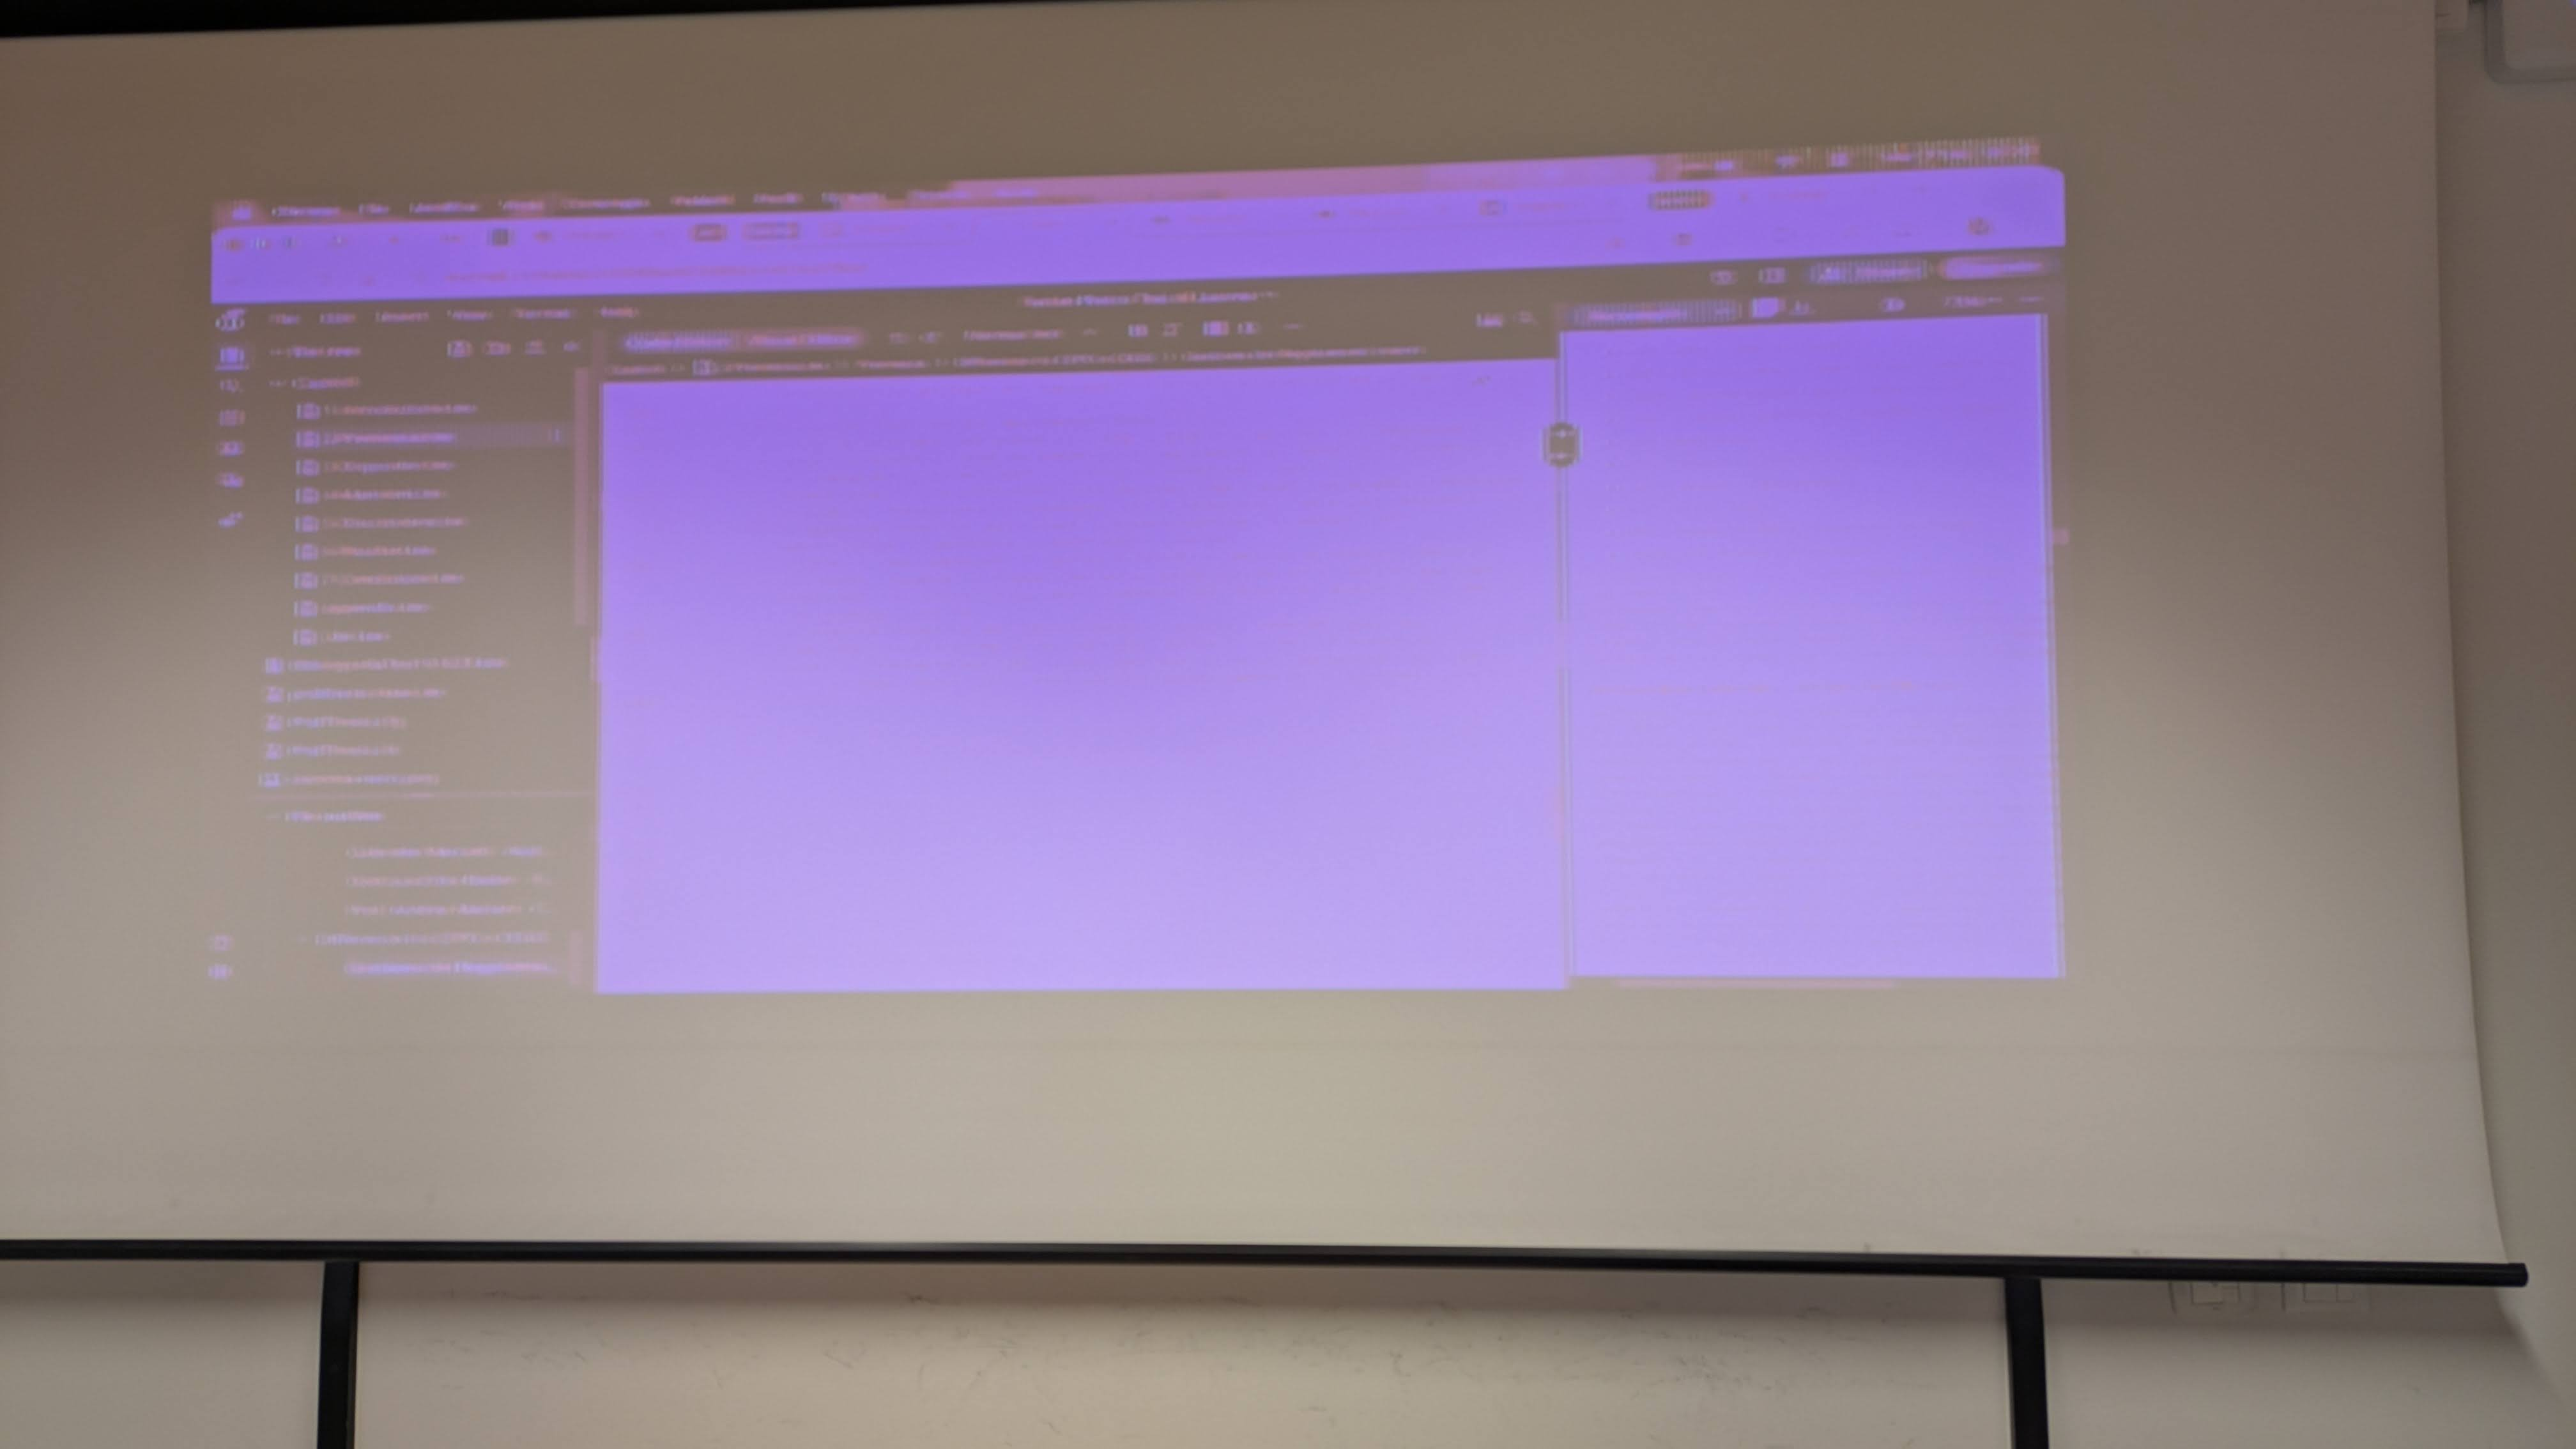
\includegraphics[width=12cm]{imgs/MagnaVGA.jpg}
                \caption{\textit{Proiettore con collegamento VGA}}
                \label{fig:VGABad}
            \end{figure}

            \begin{figure}[htbp]
                \centering
                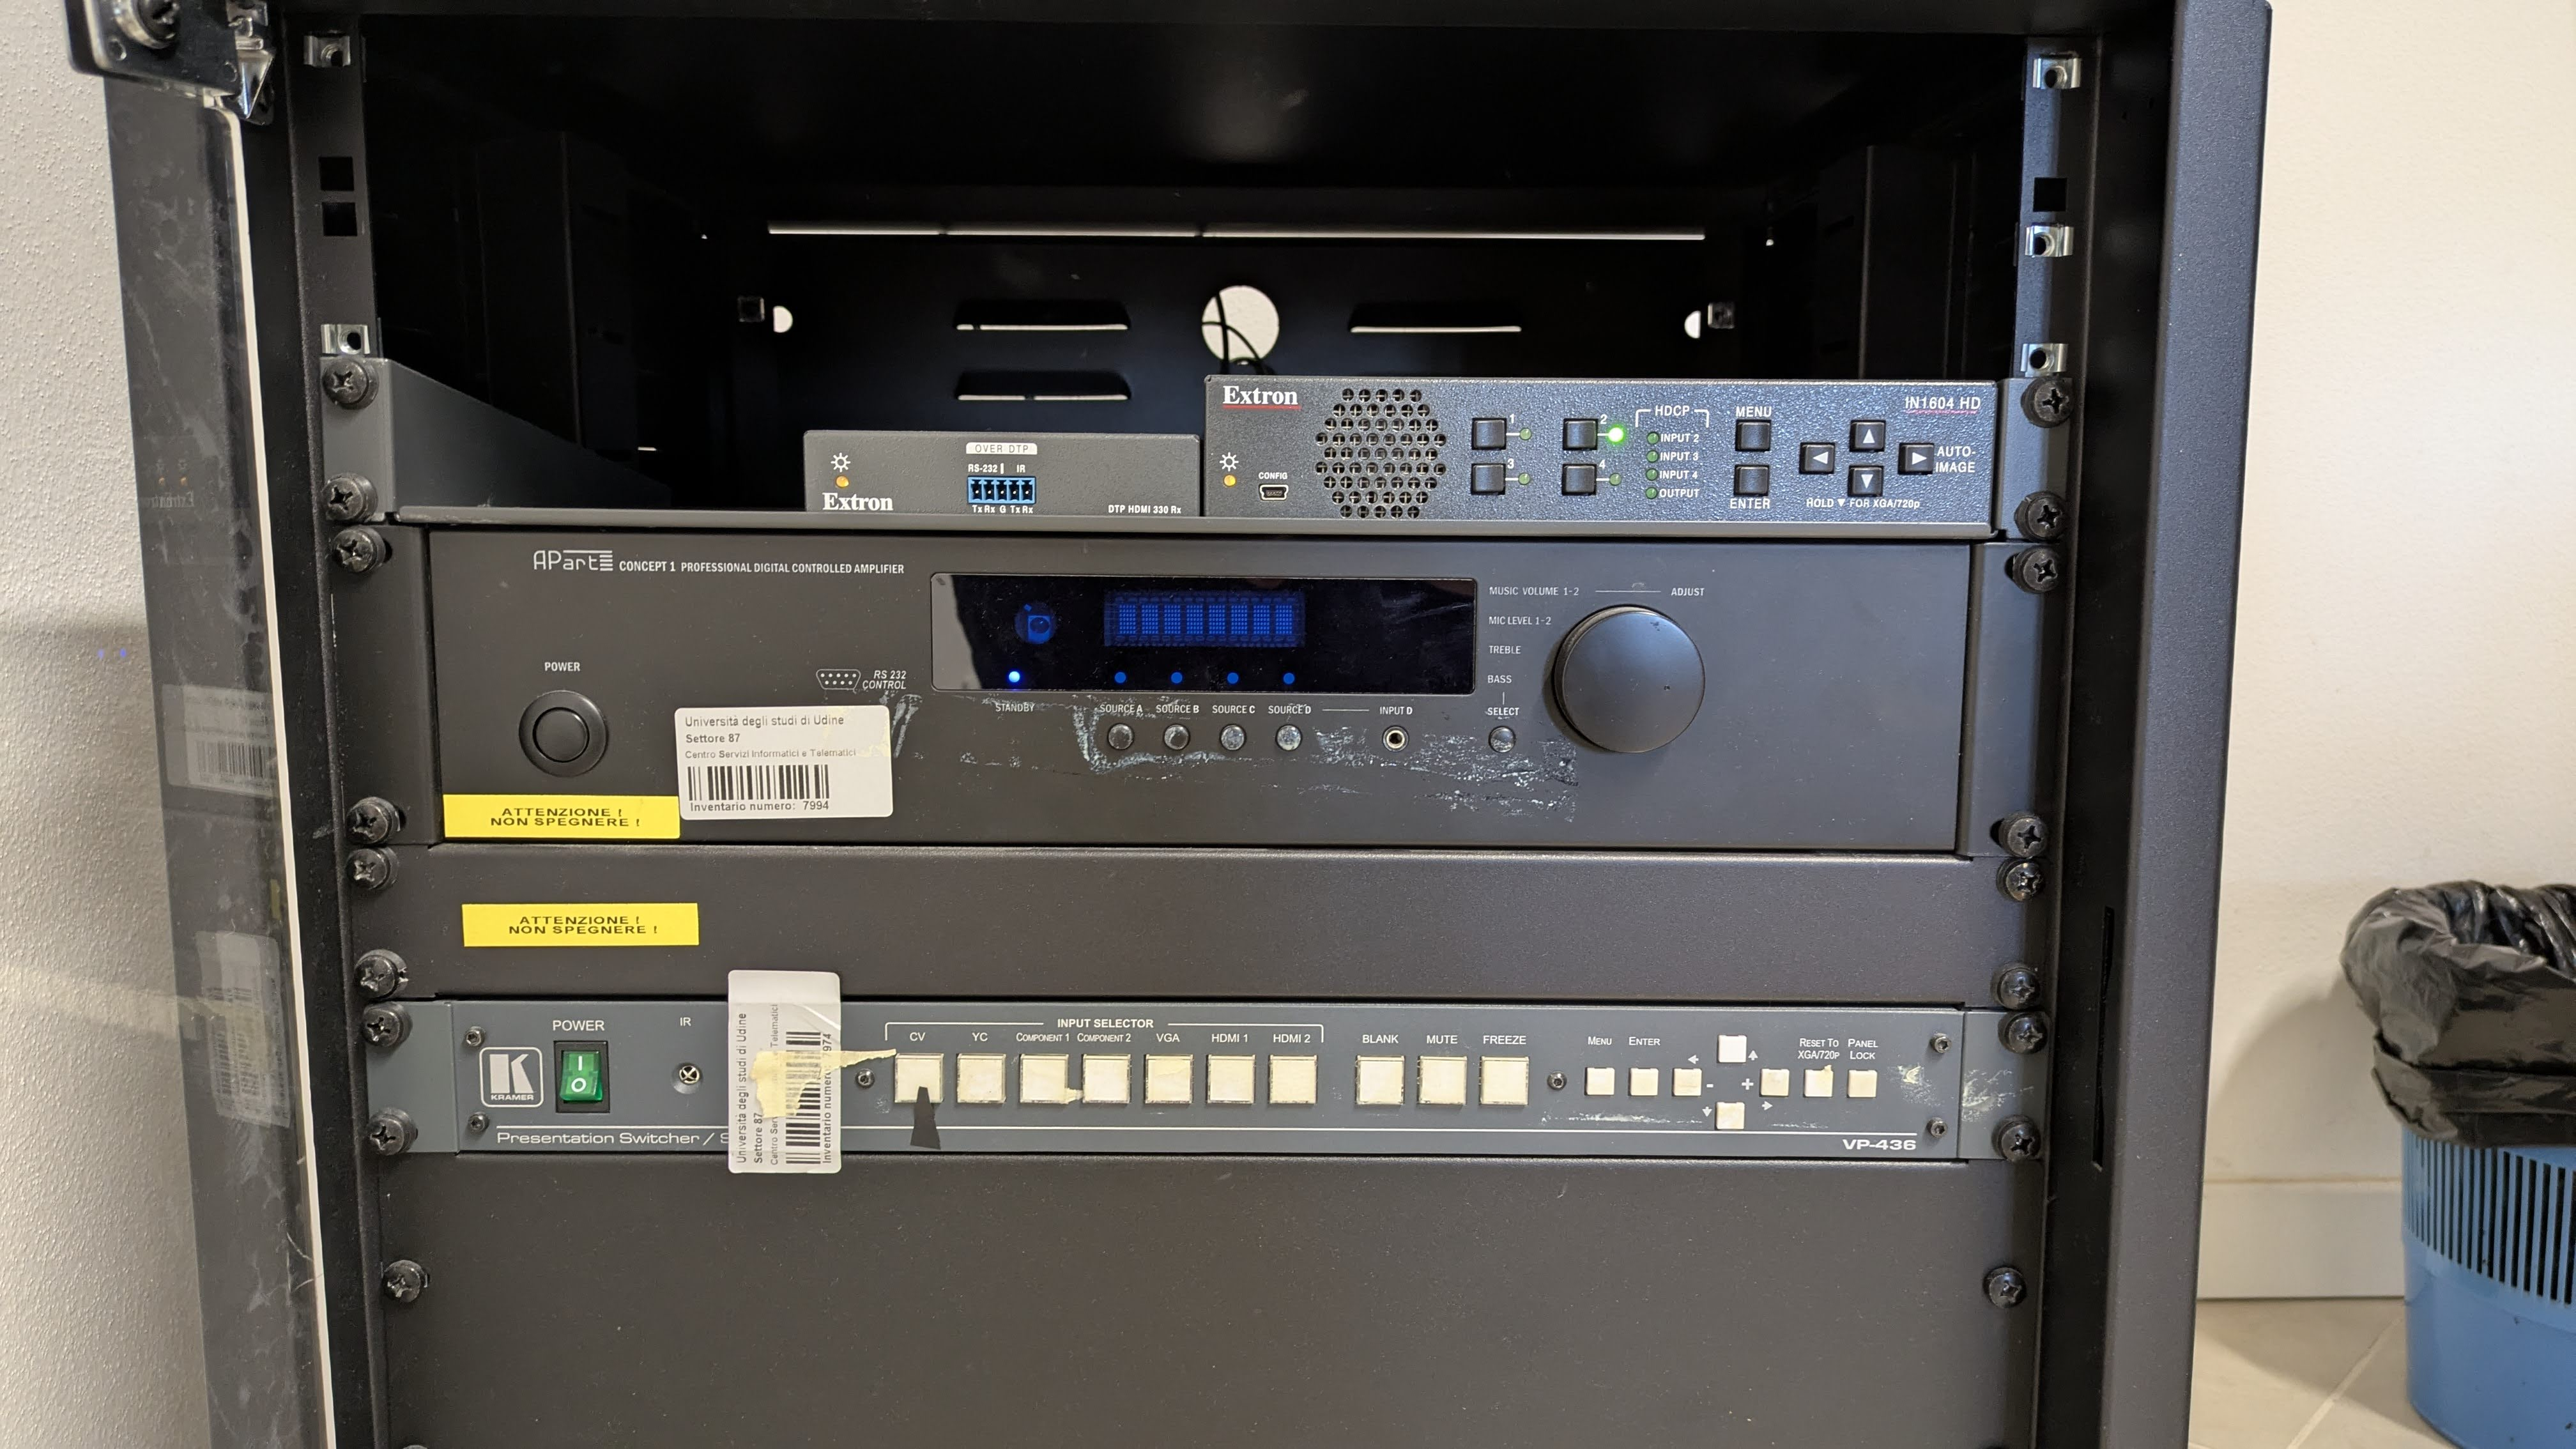
\includegraphics[width=12cm]{imgs/ArmadidettoImpiantoAudio.jpg}
                \caption{\textit{Armadietto contenente commutatore video e amplificatore}}
                \label{fig:armadietto}
            \end{figure}
    \newpage     
% ---------------------------------------------------------------------------------------
        \hfill
        \section{Altre Mansioni}
            \par
                Durante il periodo di tirocinio, mi è stato assegnato il compito di tenere traccia degli eventi costruendo, sulla base di un catalogo già esistente, un file dove si potessero segnalare i dati principali degli eventi, in modo da poter poi stipulare un report dettagliato a fine Anno Accademico. \newline
                In parallelo alla gestione degli eventi, ogni settimana per ogni giovedì, sono stato il referente per le problematiche riscontrate dalla Portineria e per le problematiche relative alla Portineria: è stato mio compito catalogare tutte le segnalazioni fatte in un file preesistente, gestito dalla Dirigente Amministrativa; questo file è stato compilato e quindi spedito a chi di competenza con cadenza settimanale. 